A rectenna receives electromagnetic power with antenna and convert it to electric power with rectifier. Diverse configurations are available for energy harvesting, such as \textit{Schottky} \cite{Akkermans2005, Boaventura2013}, \textit{CMOS} \cite{Stoopman2014, Valenta2014}, \textit{series} \cite{Georgiadis2011, Collado2013}, \textit{shunt} \cite{McSpadden1998, Guo2012}. Interestingly, those models are not equally suitable for the same input power, and maximizing the rectenna efficiency ${e_3}$ requires a proper selection according to the power range. As reported in \cite{Valenta2014, Costanzo2016}, low barrier Schottky diodes are commonly used for input power between 1~\muW and 1~mW. Specifically, single diode is preferred for low power below 500~\muW and multiple diodes are typically applied for input power above 500~\muW \cite{Clerckx2019}. Hybrid designs as \cite{Sun2013} may be employed to maintain a high efficiency for large power range.

Besides the rectenna circuit, the shape of the received signal also influences the RF-to-DC efficiency ${e_3}$. It was first demonstrated in \cite{Trotter2009} that multisine waveform \textit{i.e. Power-Optimized waveform (POW)} outperforms the single tone waveform \textit{i.e. Continuous Wave (CW)} in operation range and power efficiency. The expression of a multisine waveform with $N$ subcarriers writes as a summation of $N$ sine waves:

\begin{equation}\label{eqn:multisine}
  {V_{{\text{multisine}}}}(t) = \sum\limits_{n = 0}^{N - 1} {\frac{1}{{\sqrt N }}} \sin \left( {2\pi \left( {{f_{\text{0}}} + n\Delta f} \right)t} \right)
\end{equation}

where ${{f_{\text{0}}}}$ is the minimum frequency and ${\Delta f}$ is the spacing. Figure \ref{fig:waveform_comparison} \cite{Trotter2009} illustrates the three-subcarrier case for both signals in time and frequency domains. It can be observed that multisine waveform provides a higher PAPR equals to ${\sqrt N }$ and occupies a bandwidth of $(N - 1) \Delta f$ with the same average power as CW, which is equally distributed to its components. 

\begin{figure}
  \centering

  \begin{subfigure}{.5\texiwidth}
    \centering
      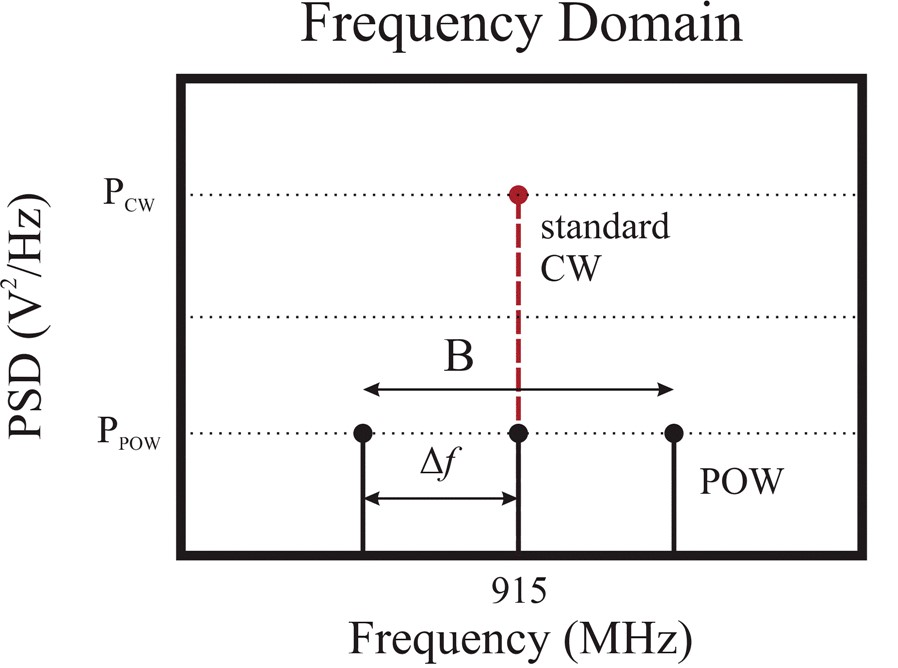
\includegraphics[width=0.5\textwidth]{Frequency domain comparison of a typical 3-subcarrier multisine and CW}
    \caption{Frequency domain}
    \label{fig:frequency_domain}
  \end{subfigure}

  \begin{subfigure}{.5\texiwidth}
    \centering
      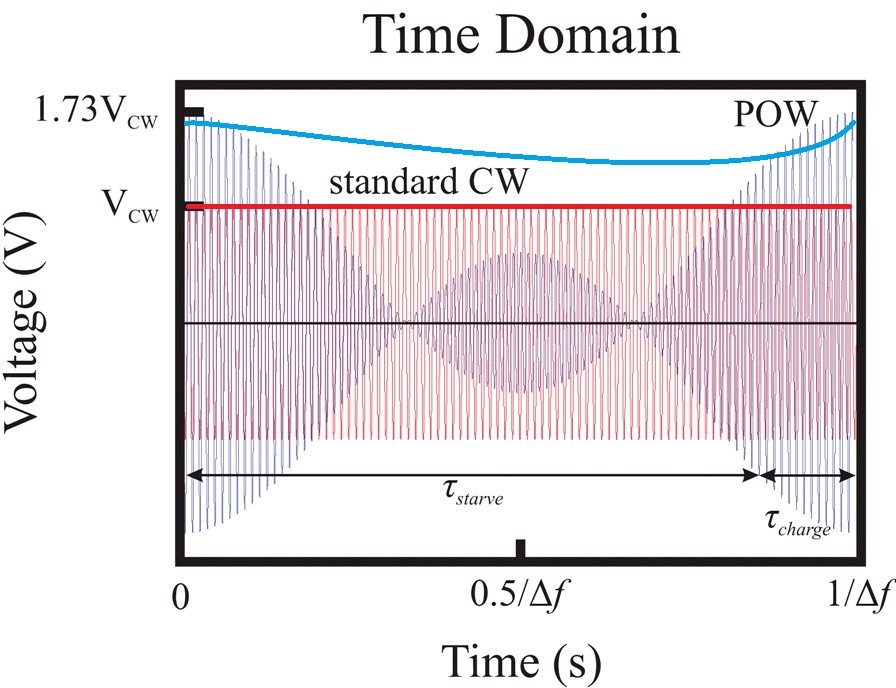
\includegraphics[width=0.5\textwidth]{Time domain comparison of a typical 3-subcarrier multisine and CW}
    \caption{Time domain}
    \label{fig:time_domain}
  \end{subfigure}

  \caption{Comparison of a typical 3-subcarrier multisine and CW in time and frequency domains (modified from \cite{Trotter2009}). The thick lines are examples of rectifier output voltage.}
  \label{fig:waveform_comparison}
\end{figure}

The advantage of multisine in WPT is that the high PAPR increases the peak rectifier output voltage. With a proper signal and circuit design, high voltage may be preserved during the cycle if discharging is slow enough, as indicated by the thick blue line in Figure \ref{fig:time_domain}. To enhance the RF-to-DC efficiency ${e_3}$, a large number of tones may be used to increase PAPR, and the multisine signal will appear as pulses with period of $1/\Delta f$. Most of the signal power will be concentrated in those pulses to trigger the diode and charge the capacitor. However, more subbands lead to smaller frequency gaps and longer charging cycle when the bandwidth is fixed.





























In this article, we employ a simplified rectifier model proposed by [Waveform Design] that captures the fundamental diode nonlinearity in the presence of multi-carrier unmodulated (multisine) and modulated excitations. As illustrated by Figure {equivalent_circuit}, the rectifier consists of a single diode as the source of nonlinearity and a low-pass filter to store energy. It is proved in [A Low-Complexity] that this analytical model is suitable for more complicated circuits as voltage doubler and diode bridge rectifiers. 